\section{Design}
  \label{sec:Design}
  \subsection{Overall Design}
Linux container technology like Docker enables consistent software and hardware environment for development, build and deployment. By developing using Docker, developers only need to build their application once in Docker on their local machine, then the application can run on any Docker-enabled machine. However, Docker is not usually installed on current HPC systems. The main reason behind it is that Docker requires Linux kernel version to be higher than 3.8, but current main stream HPC system have lower kernel version. For compatibility and security consideration, it would take years before HPC systems can upgrade their Linux kernel. Existing solution on current HPC systems either requires specially customized HPC system or Docker daemon. However, those customizations would limit the practicability to deploying such system to other machines. First, most HPC systems are not allowed to be customized either in software or hardware by normal users. Second, customized Docker daemon could bring compatibility and security issues. 
  
To overcome the Linux kernel version issue and provide more flexible design environment, we first create a extra virtual machine layer on top of the host and then deploy Docker on the virtual machine layer as shown in \textbf{figure \ref{bee-framework}}. Besides brings standard latest Docker to HPC system, the addition virtual machine layer also brings following advantages: (1) Since we have full control in the virtual machine, we can create consistent environment for upper Docker layer across platforms. For instance, we can also deploy BEE on both HPC and commercial cloud computing system (e.g. AWS), which allow Dockerized HPC applications to run on unmodified. (2) Docker only brings virtulization on software/OS level. The additional virtual machine layer brings extra hardware level virtulization, which further ensure long-term reproducibility. (3) Docker level live migration requests hosts(in prospective of Docker container) OS version to be similar between checkpointing side and restoration side. This extra virtual machine can guarantee that requirement is met. This can be a problem if Docker is run directly on the hosts.   

\begin{figure}[h]
    \centering
    \caption{BEE Framework}
    \label{bee-framework}
    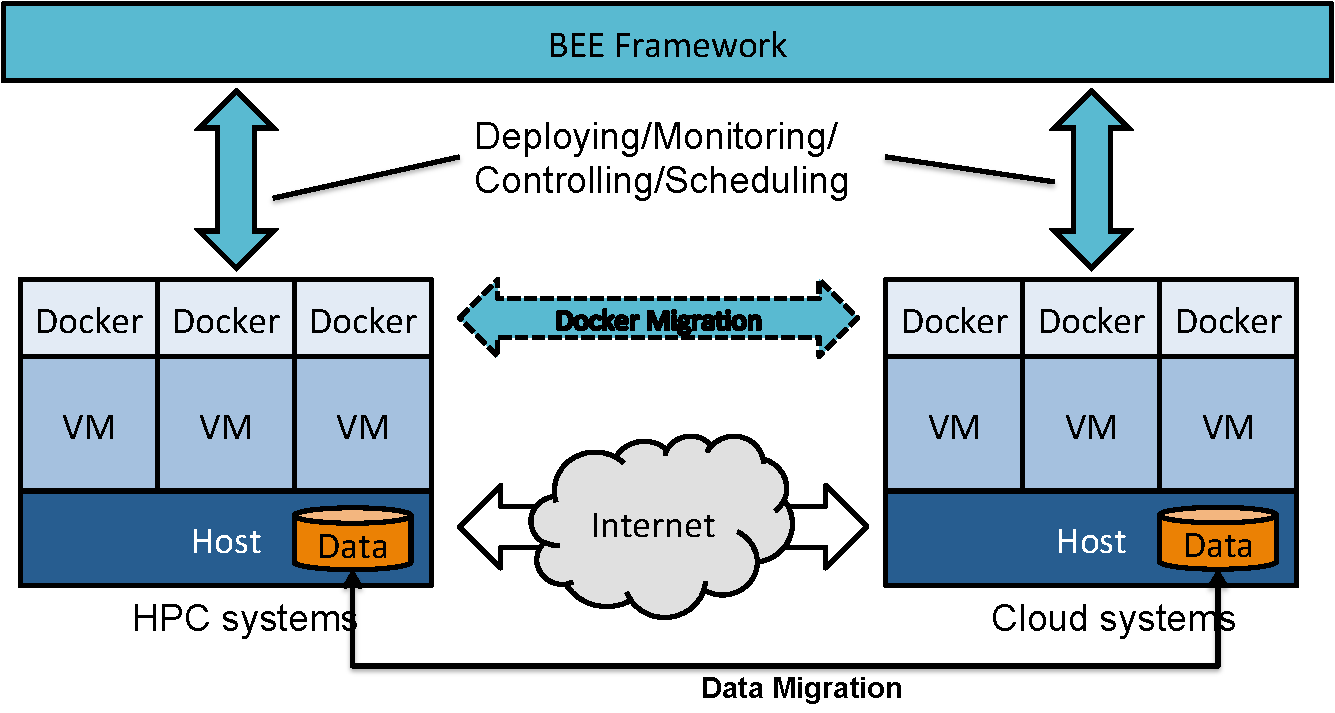
\includegraphics[width=0.5\textwidth]{figures/bee-framework.pdf}
\end{figure}
 
\subsection{Network Design}
In this section, we discuss our network design in \texttt{BEE}. Network part of \texttt{BEE} is mainly used for two functions. The first one is that we need to dynamically configure and do deployment in virtual machine and Docker container. This need to be down automatically and remotely. Also, since we are aiming at HPC application and most HPC application requires MPI, so that we also need to build network for MPI communication between different computing nodes. For the controlling virtual machine and Docker, we choose to use Secure Shell(SSH). It has several advantages: (1) SSH server and client can be easily deployed on most machines and it is usually enable on HPC systems; (2) RSA key pairs can be used to for simple and secure machine control without worrying about complicated password; (3) SSH allows remote command execution without login, which can facilitate batched virtual machine/Docker control. Basically, we need to run SSH server inside virtual machine and Docker container. To avoid port conflicting, we configure the SSH server to listen to different ones than the host, since HPC won't allow normal user to configure SSH port. As for the MPI communication, we need to create a virtual subnet comprises all virtual machine or Docker container, so that they can communicate.

\subsubsection{Virtual machine layer}

First, we design the network between virtual machine. This is necessary since the Docker layer on top of it would depends on the network here. The main challenges of designing network for virtual machine is configure virtual network card without root privileges, since that is the most common case for HPC users. We designed two solutions for different hardware configurations on the HPC systems.

To connect virtual machine to the host network, many commonly used approaches requires root privilege. However, in this work, we restrict our scope to only use normal user level privilege, so we do not consider technologies like TAP in our design. In order to enable SSH connection to the virtual machine through host, hypervisor much be configured to use port forwarding to map an unused port on host to the SSH port on the virtual machine. However, this makes the network interface card(NIC) unusable for MPI. Although some MPI libraries can be configured to use designated port and can cooperate with port forwarding, many commonly used MPI libraries (e.g. OpenMPI) uses random port, which is not easy to work with port forwarding mechanism. So, we build a second virtual NIC dedicated for MPI communication. We design three solutions to cooperate virtual NICs with physical NICs on the host. 

\textbf{Solution 1: 2 NICs}
We design our first solution on the 'Galton' nodes of our testbed cluster machine. Each Galton node has two physical NICs. So, we use the port forwarding combining the SSH virtual NIC with one physical NIC and use simple pass-through mode to combine the MPI virtual NIC with the other physical NIC. This is the simplest design in our three solutions. However, this solution is limited to deploy on computing nodes with multiple physical NICs. 
\begin{figure}[h]
    \centering
    \caption{Network Design using two NICs}
    \label{2nic}
    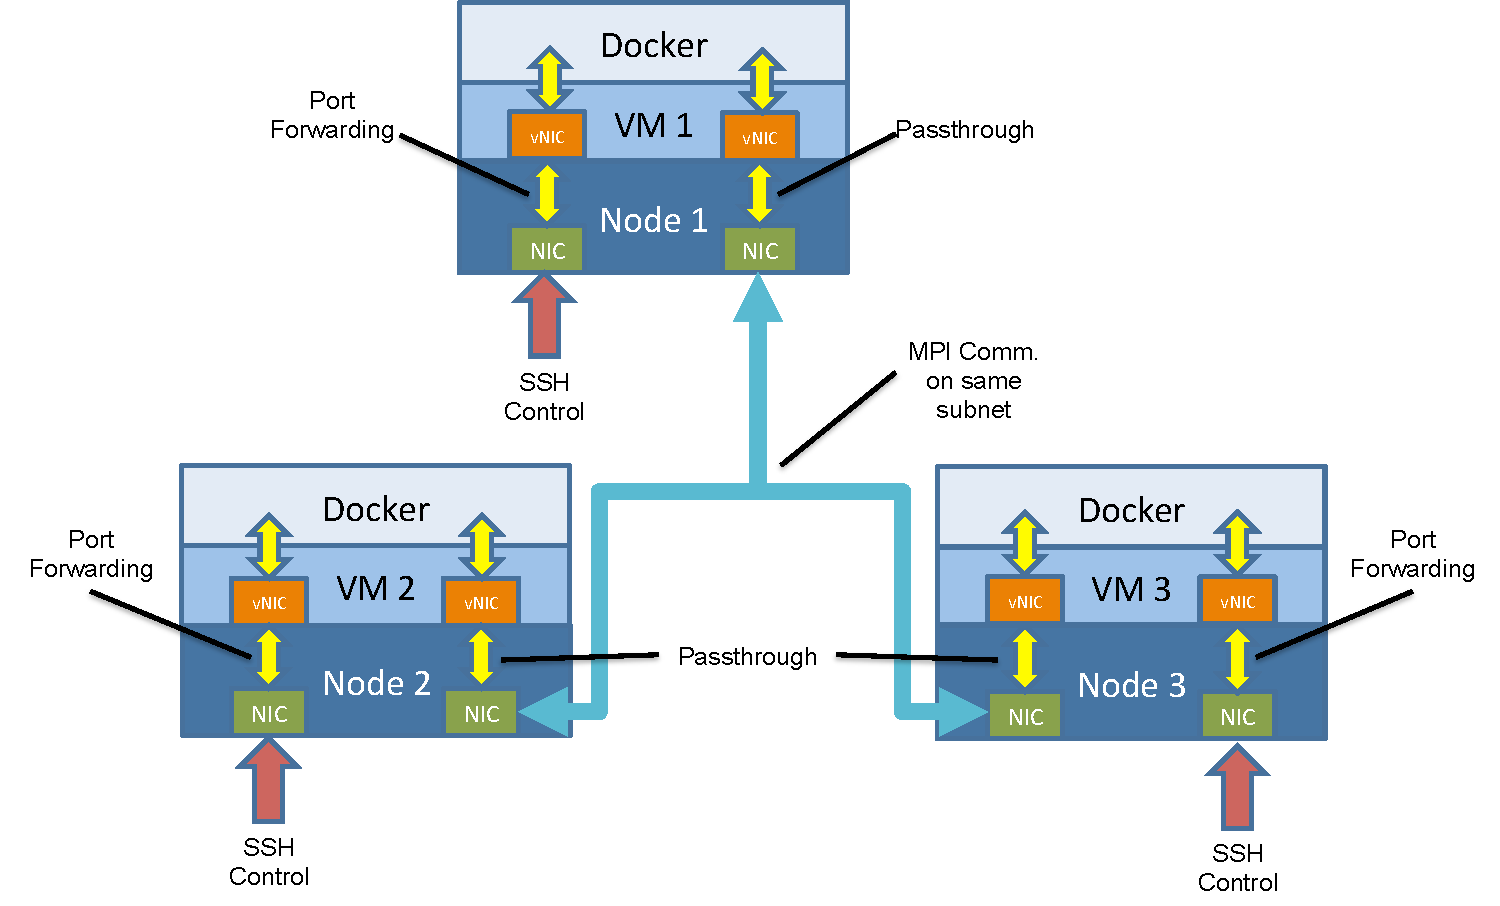
\includegraphics[width=0.5\textwidth]{figures/2nic.pdf}
\end{figure}
 
\textbf{Solution 2: 1 NIC + multi-cast}
To accommodate more general case, in which each computing node has one physical NIC, we design our second network solution. In this solution, we still use port forwarding to combine the SSH virtual NIC with the physical NIC. For the second virtual NIC for MPI, we use multi-cast subnet to connect all second virtual NICs of all virtual machines together. Since all virtual NICs are connected to the same subnet, there is no restriction on port usage, so any MPI library can be used. The advantages of this design is that the configuration is simple and if one node in the multi-cast network failed, it won't affect the connect in between other nodes, which can cooperate with simple fault tolerance mechanism. However, multi-cast network also brings higher communication overhead. Although MPI broadcast communication behaves similar in the multi-cast subset, point-to-point MPI communications are converted to multi-cast, which generated more data packages in the subnet.
\begin{figure}[h]
    \centering
    \caption{Network Design using one NIC and multicast}
    \label{mcast}
    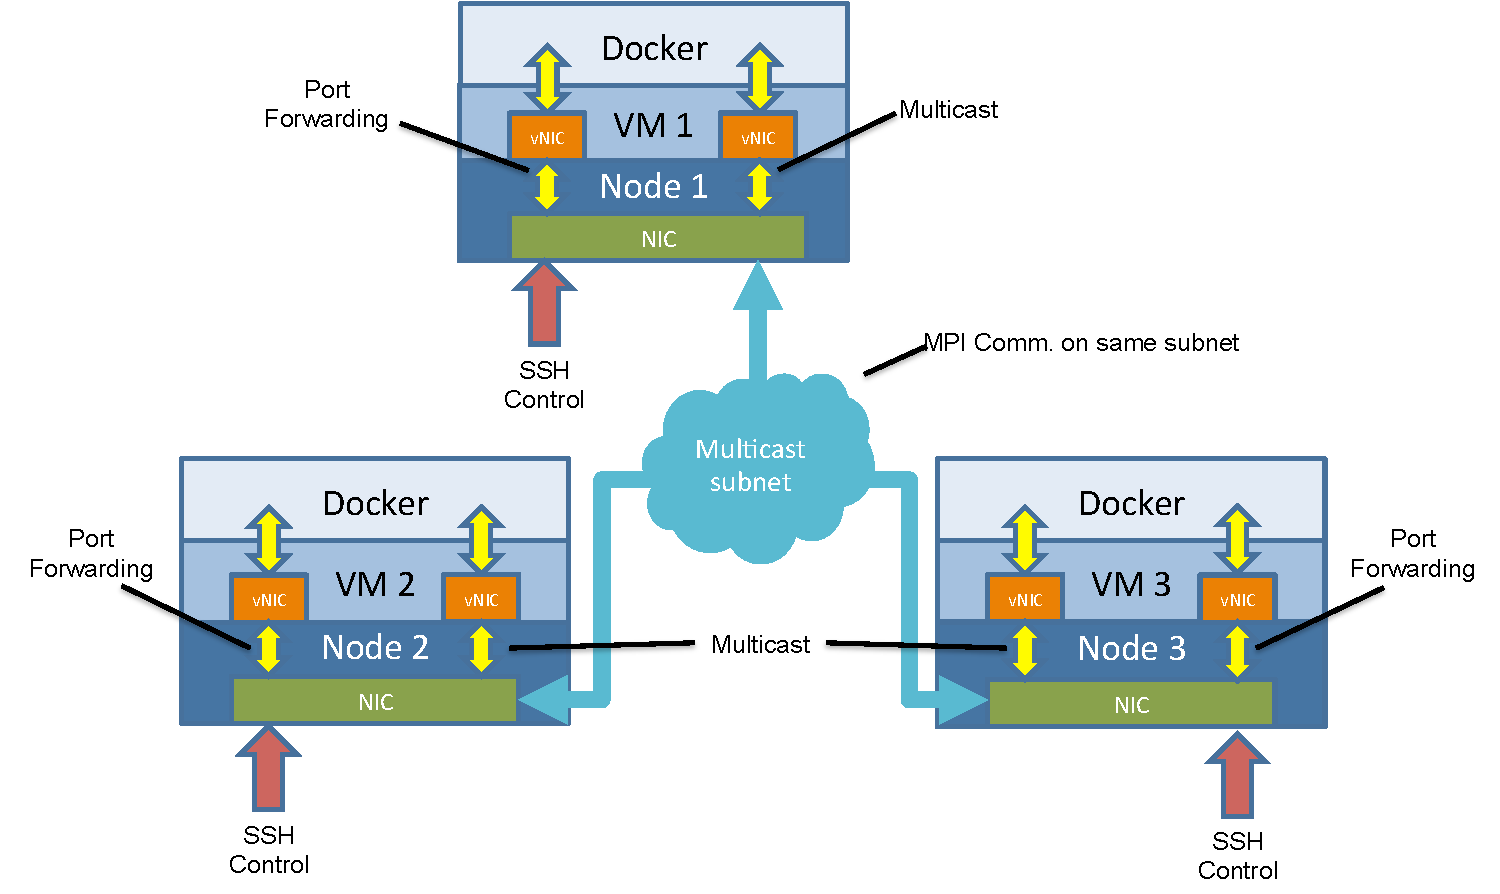
\includegraphics[width=0.5\textwidth]{figures/mcast.pdf}
\end{figure}
 
\textbf{Solution 3: 1 NIC + P2P sockets}
To keep using one physical NIC and reducing network communication overhead, we design our third solution. Different than our second solution, instead of connecting the second virtual NIC to a multi-cast subnet, we connect each second virtual NIC from each virtual machine using point-to-point socket connection. This is similar to the wired Ethernet connection between computing node in HPC system. Since there is point-to-point routing path between nodes, there are no extra unnecessary data packages in the network. However, socket connects between nodes may route via inter-median nodes, so if one node fails, it may breaks several connects multiple node, so more complication fault tolerance mechanism need to be adopted. Also, the performance of this kind of network is affected by the connection pattern between nodes, so we adopt two connection pattern in this solution. 

\begin{figure}[h]
    \centering
    \caption{Network Design using one NIC and P2P sockets}
    \label{p2p}
    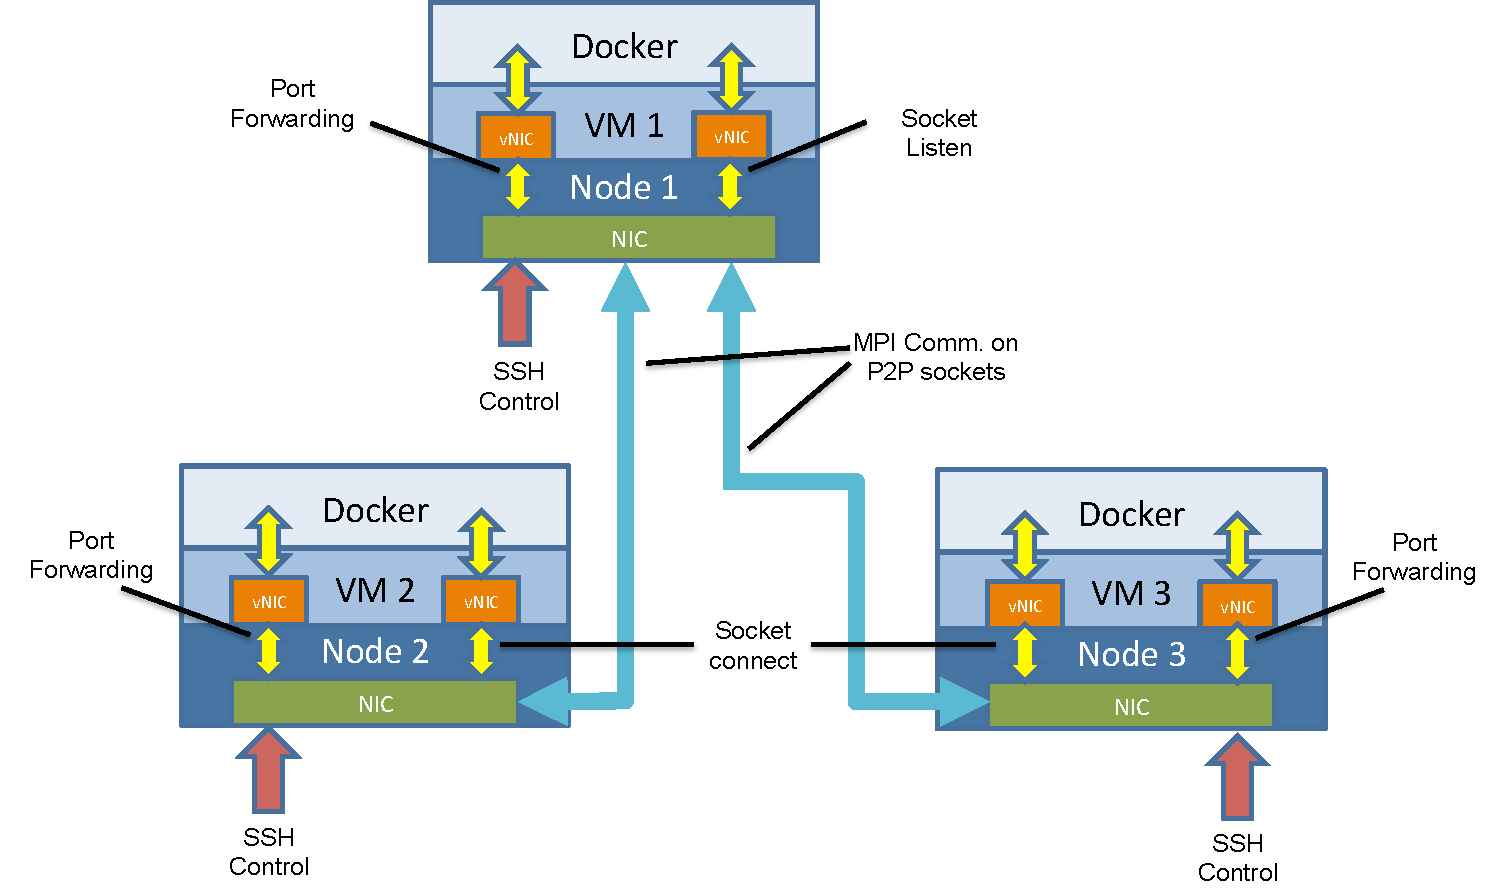
\includegraphics[width=0.5\textwidth]{figures/p2p.pdf}
\end{figure}

\begin{enumerate}
\item \textbf{Star-shape connection}
We first connect the nodes in start-shape with master node in the center. This connection pattern can effectively limit connection hops between each pair of nodes. However, since all communications must go through the center node, it may become a hot-stop in the network especially for application involves intensive network communication or the shared storage design needs network communication(will be discussed in later section).
\item \textbf{Tree-shape connection}
Then we connect nodes in tree-shape which master node as the root. especially, we use binary tree structure. This connection can mitigate hot-stop issue, but it also more connection hops between each pair of nodes.
\end{enumerate}

\subsubsection{Docker container layer}
Based on the network of virtual machine layer, we now design the network between Docker container. There are several network configuration for Docker container. To minimize network overhead, the most direct way is network pass-through. Basically, all network interfaces on the host (i.e virtual machine in our case) will be exposed to Docker container. Since there is not additional buffer or translation in between, it usually bring the lowest overhead. However, it is also considered to be the least unsecured since everything is exposed. But we build Docker inside virtual machine, this extra layer already provide enough isolation, so there is no extra security issue there. So, we choose pass-through as the network mode used for Docker container(i.e. host mode). Since network interface is exactly the same between virtual machine and the Docker container inside it, the software level configuration (e.g. SSH, MPI) are similar and easy to configure.

\subsection{Storage Design}
In this section, we design the share storage system of \texttt{BEE}. General HPC application usually use some kind of shared file system(e.g. NFS) to share data between processes. To provide the same environment, we need to build a shared file system across different nodes in \texttt{BEE}. To between integrate user's work-flow logic, we aim to separate data from run-time data and operation system itself. This separation allows users to easily migrate their data to other platform without extra space overhead. We design three architectures to allow different processes in different nodes to share files in real-time.

\subsubsection{Extra Data Image + NFS}
In our first solution, we build an extra data image and mount it as the second disk. Due to the copy-on-write characteristic of most virtual images, filed updated by one machine is visible by other machine in real-time. So, we choose to mount this data image only to the master node, and use NFS to share mounted disk with other virtual machines. By using the extra data image, data can be easily migrated. The input data is first pre-loaded in the image, which can result from other part of user's work flow. After execution, the output data is also stored in this image. To move the data to other part of the work flow, user only need unmount the data image from current computing node and mount to the computing node used for the next stage. Also, the image encapsulation can protect data integrates. However, the data image is shared with other worker nodes via NFS, which highly depends on the performance of virtual network. If user's application is I/O extensive and the network bandwidth is limited, it may consume too much network resource, which may degrade MPI communication performance and slows down users application.
\begin{figure}[h]
    \centering
    \caption{Shared Storage Design using Extra Data Image + NFS}
    \label{fs1}
    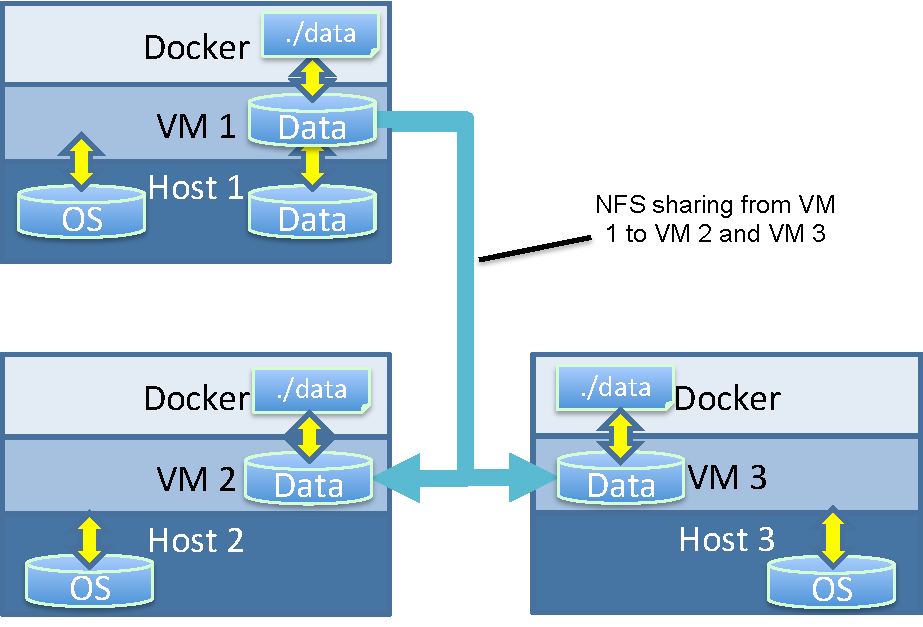
\includegraphics[width=0.4\textwidth]{figures/fs1.pdf}
\end{figure}
\subsubsection{Only NFS}
In our second solution, we aim to reduce the dependency on virtual network. Instead of building our own NFS sharing environment, we use the NFS server that is commonly used in most HPC system. Each virtual machine mount to the same directory on the host node. Data in the same directory is shared between different host node via fast dedicated NFS system. Since only the host directory is mounted, the data is also accessible during the execution, which can be used for output monitoring or sampling for in-situ analysis. This is not possible if we use the first solution, since data is not accessible outside the data image. This solution only relies on the network between host and virtual machine, which saves most virtual network bandwidth for MPI communication.
\begin{figure}[h]
    \centering
    \caption{Shared Storage Design using Only NFS}
    \label{fs2}
    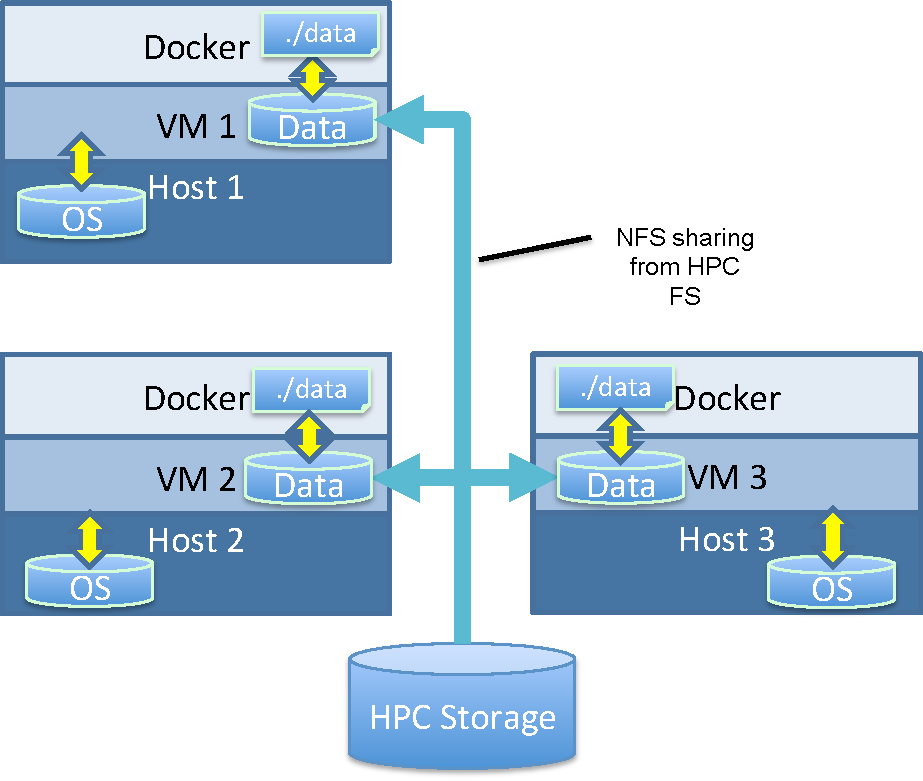
\includegraphics[width=0.4\textwidth]{figures/fs2.pdf}
\end{figure}
\subsubsection{Virtual IO}
In our third solution, we eliminated all the dependency on virtual network. We use the virtual IO \cite{russell2008virtio} feature in QEMU to map a host directory to a directory in virtual machines. It only required minimum configuration at virtual machine boot time. Similar to solution 2, each machine are mapping the same directory, so the data is still shared using NFS system in HPC system and it is visible to the host in real-time. Since it does not relay on network, the whole virtual network is saved for MPI.
\begin{figure}[h]
    \centering
    \caption{Shared Storage Design using Virtual IO}
    \label{fs3}
    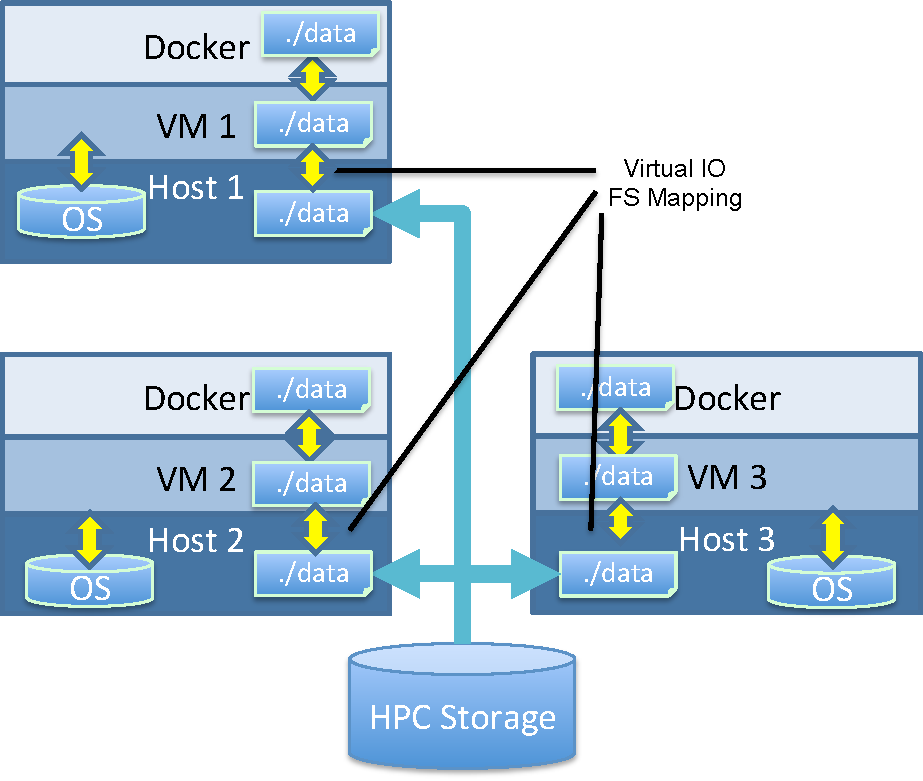
\includegraphics[width=0.4\textwidth]{figures/fs3.pdf}
\end{figure}
\subsubsection{Data sharing between Docker containers}
Finally, as for data sharing in Docker layer, we use the data volume sharing feature in Docker to mount the shared folder in virtual machine to a directory in Docker. Since Docker runs as process in virtual machines, sharing data in between brings negligible overhead. This configuration is also compatible with all three data shared mechanism in virtual machine layer.

\subsection{BEE-VM Image Builder}
Besides network and shared storage design, designing virtual machine image also plays an important role in \texttt{BEE}. Virtual machine is the core of \texttt{BEE} that combines computing resources from host, virtual network, shared storage, user provided Dockerized application and Docker container management together. Customizing virtual machine image is the key for \texttt{BEE}. For uniform standard image building process, we design our \texttt{BEE-VM} Image Builder using Packer \cite{packer}. Packer allows us to build customized image automatically. We can also run our own configure scrips in the virtual machine image to enable more flexible customization. Although it is also possible to configure and customize virtual machine OS after booting virtual machines, customize and configure images off-line can save a lot of time. For example, building and installing packages. We aid to minimize on-line configuration as much as possible to reduce \texttt{BEE} deploying time and leave most of the work to \texttt{BEE-VM} Image Builder. The main customization responsibility of \texttt{BEE Image Builder} include:
\begin{enumerate}
\item \textbf{Create and configure user:} We need to create a user for the host to login or control the virtual machine.
\item \textbf{Configure network interfaces:} Network interface must be configured in advance before \texttt{BEE} can configure and control the virtual machine after it has started. However many network configuration cannot be determined until boot time, so we design a customize script built in to the image, so that network interface can be customized automatically when the virtual machine started.
\item \textbf{Configure SSH server/client:} SSH is required for \texttt{BEE} to control virtual machine and it is also important for MPI. So, we need to configure SSH key pairs and customized port number in this step.
\item \textbf{Install essential packages and tools:} Many packages and tools are required including MPI and Docker.
\item \textbf{Configure proxy settings:} Most institutional HPC system requires some kind of proxy setting in order to connect to the Internet. 
\item \textbf{Configure shared storage:} We need to pre-configure the virtual machine image for mounting shared storage system. For example, configuring NFS server.
\end{enumerate} 

\subsection{Work Flow Integration}
%\jchen{explain how we can integrate work flow logic in to \texttt{BEE}}
By encapsulating each components of HPC or cloud computing system into container, each component can be treated as modules that can be easily assembled into a large system as needs. This enables user to easily build their work flow logic into BEE. Once user has set the work flow logic, BEE will automatically deploy and manage users application according to the logic. For example, as show in \textbf{Figure \ref{workflow}}, when user wants to a series of pipelined simulations, the user need to manually configure and start each simulation one by one and also need to handle data transfer for the pipeline logic. If the pipeline consists many simulations, it can be considerable hard to manually deploy and debug, especially when different simulations are conduced on different hosts. However, by using BEE, user only need to indicate which simulations need to run and which one follow the other, then BEE can automatically deploy simulation applications in order and setup the pipeline data transfer. The containerized environment also allows user to change certain part work flow logic at runtime as long as it does not interrupt normal execution. For example, if during the pipelined simulation, some bug occurs and causes incorrect final output data. In-situ analysis is a common approach to diagnose the problem by checking intermediate result between two simulation. User need to login to each hosts and manually deploy some in-situ analysis tools, which can be hard when the original work flow logic is complication. By using BEE, the in-situ analysis tool can be encapsulated as another user application and is able to be deployed into users work flow at real-time.

Continues Integration(CI) has been widely used in many HPC application development process. It used for unit testing, fixing compatibility issue during integration, etc. Many development project choose to use standard Docker image as output application format. Since BEE takes standard Docker image as input, it can seamlessly interfacing CI development.
\begin{figure*}[h]
    \centering
    \caption{BEE with Workflow Integration}
    \label{workflow}
    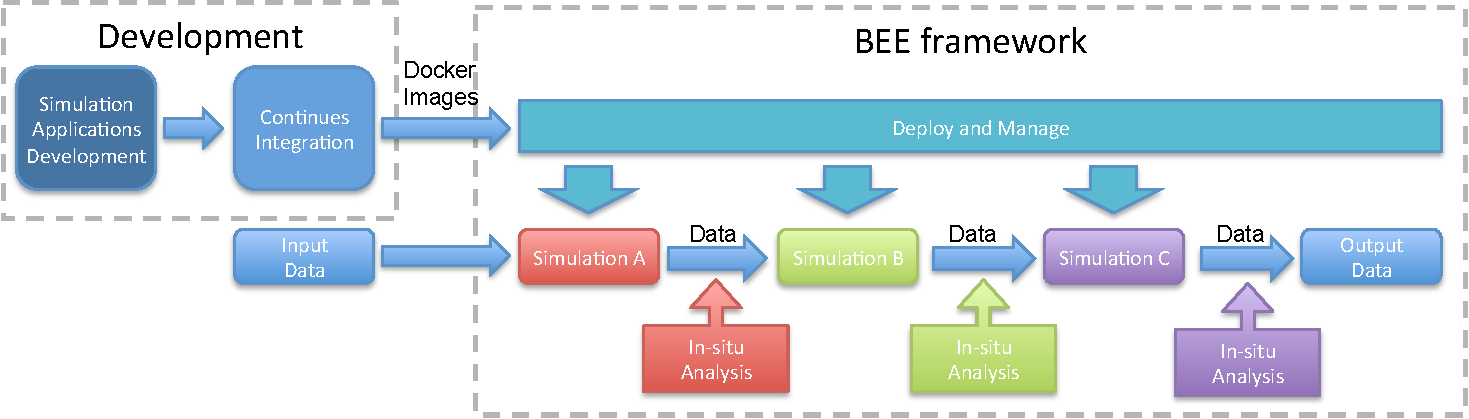
\includegraphics[width=0.9\textwidth]{figures/workflow.pdf}
\end{figure*}

%\subsection{Live Migration} % changed by qguan : live migration means something else rather than we are using.
\subsection{Application Migration}
An allocated a time slot for each execution on HPC system is usually not enough for a whole execution. Once a user's allocation is near end, the user must take a checkpoint of the application to avoid lost of progress. Then, the user can choose whether to wait for another time slot or manually migrate to another HPC system. However, it imposes several challenges: First, checkpoint feature is not available in HPC applications. Developing checkpoint/restoration requires extensive programming efforts. Second, due to the intrinsic characteristic of computing pattern of HPC applications, taking a checkpoint anytime is not always possible. For example, large scale application usually process stage by stage. Checkpoint in the middle of a stage is difficult since it is hard to store complicated status information during the computation. Checkpoint is only possible in between stages. However, if current time slots is not enough to finish the current stage, it can be in serious trouble. Third, migrating to a different HPC system can be difficult due to different software and hardware configuration. 

For better compatibility, so we integrate system level checkpoint/restoration in \texttt{BEE}. There two levels of virtualization in \texttt{BEE}, many works has been done on live migration on virtual machines between HPC system \cite{huang2007high, anedda2010suspending}, however we choose the Docker level for checkpoint/restoration since it offers several benefits. First, it allows live migration between HPC and cloud computing system. Most cloud computing system is built on virtual machines and all hypervisors are hidden from users. So, checkpointing and restoring in the virtual machine level is not possible for normal users. Even if some cloud offers checkpointing feature, the checkpoint format may incomparable with the one on HPC system, since they may use different kinds of hypervisors. Second, system level checkpoint is usually considered to has high storage overhead and high time cost \cite{voorsluys2009cost}. However, Docker level checkpointing/restoration \cite{criu} is done in the process level. The check-pointing process is fast and light-weight. The checkpoint size is almost the memory usage size of the current running application, which can be easily migrated across different platforms. Third, Docker level migration can solve the compatibility issue in application level checkpointing.
\subsection{Hybrid HPC and Cloud BEE Framework}

In this section, we discuss the overview of our BEE framework. Besides HPC computing resources, we also aim to utilizes computing resources from cloud environment. Efficiently manage available resources and deploying virtualized execution environment is one of the keys for providing high performance virtualized environment \cite{huang2006case, mateescu2011hybrid}, so we design the BEE framework to efficiently manage our multi-layer virtualized environment.  As shown in \textbf{Algorithm \ref{bee}}, we outline the general workflow of BEE. First, user need to provide all the computing resources available to that user. This can be both HPC system and cloud computing system. User need to indicate which nodes are available and current allocated time slot. User also need to indicate the priority of using these computing system. For example, when running a compute intensive application, user may want prioritize system with high performance to the front of the list. Then user need to provide their Dockerized application with input data and hardware configuration file indicating on what kind of system they want their application to run. 

Before execution, BEE picks the system from the front of the list(\textbf{Line 3}), which has the highest priority. Then it check if current application is in initial stage or needs to restore from previous checkpoint. If it is in initial stage, BEE just attach the input and run the application as shown in \textbf{Line 10 and 13}. Otherwise, BEE first migrate previous intermediate data and checkpoint from last system to current one (\textbf{Line 5 and 6}) then attach the data and restore Docker checkpoint (\textbf{Line 7 and 8})before running. 

During execution, BEE monitor the current state of the running BEE cluster. When it is closing to the end of current time slot, BEE checks if current application has completed its execution. If so, BEE stops the cluster and output the result. Otherwise, BEE initiate checkpointing procedure. It first pause current execution to take a checkpoint of each Docker container and detached the intermediate data. It marks $need\_migration$ has true to ensure the current application will resume from current execution stage next time. When finish checkpointing procedure, BEE will check for next available system to run. If no other computing system available, BEE will store current data and checkpoint data in disk, until user indicate new computing resources are available.
	

\begin{algorithm}
\caption{BEE Framework}
\label{bee}
\begin{algorithmic}[1]
\REQUIRE{$HPC/Cloud_1$: [Host nodes: $H_1$, $H_2$,..., $H_k$][Time slot: $T_1$]}
\REQUIRE{$HPC/Cloud_2$: [Host nodes: $H_1$, $H_2$,..., $H_k$][Time slot: $T_2$]}

{...}

\REQUIRE{$HPC/Cloud_m$: [Host nodes: $H_1$, $H_2$,..., $H_k$][Time slot: $T_3$]}
\REQUIRE{Computing resource priority list: $L$}
\REQUIRE{User Dockerized application(Docker image/Dockerfile)}
\REQUIRE{Input data: $D$}
\REQUIRE{User defined hardware configuration: uconf}

\STATE $need\_migration \leftarrow$ False
\STATE $lastHost \leftarrow$ N/A

\WHILE{H $\leftarrow$ get\_top($L$)}
	\IF{$need\_migration$ is True}
		\STATE data\_tranfer($lastHost$, $H$, $D$)
        \STATE checkpoint\_tranfer($lastHost$, $H$, $DCHK$)
		\STATE attach\_data($D$, $H$) \bluecomment{Load data into H}
		\STATE mpi\_docker\_restore($H$, $DCHK$)
	\ELSE
		\STATE attach\_data($D$, $H$)
	\ENDIF
	\STATE deploy\_bee($H$, $user\_application$, $uconf$)

	\WHILE{$H$ running normal AND Running-time not close to $T$}
		\STATE Monitor($H$)
	\ENDWHILE

	\IF{execution incomplete}
    	\STATE pause($H$)
		\STATE $DCHK \leftarrow$ mpi\_docker\_checkpoint($H$)
		\STATE $D \leftarrow$ detach\_data($H$) \bluecomment{Unload data from H}
		\STATE $need\_migration \leftarrow$ True
		\STATE $lastHost \leftarrow$ H
		\STATE stop($H$)
	\ELSE
		\STATE stop($H$)
		\STATE result $\leftarrow D $
		\STATE terminate() 
	\ENDIF
\ENDWHILE

\IF{execution incomplete}
		\STATE $DCHK \leftarrow$ mpi\_docker\_checkpoint($H$)
		\STATE $D\leftarrow$ detach\_data($H$)
		\STATE stop($H$)
		\STATE store $D$ and $DCHK$ when no resource available
\ENDIF

\end{algorithmic}
\end{algorithm}


\textbf{Algorithm \ref{bee-launch}} shows the work flow in BEE used for launching BEE cluster on a given platform. Although the specific process varies from HPC system to cloud computing system, the general procedure are the same. At first, the launcher needs to know how many and which nodes are available now. Then the user Dockerized application is provided, which can be in either Docker image form or Dockerfile form. finally, user defined hardware configuration file is also provided, which is use when starting virtual machines. 

There are four stage for launching application in BEE. In the first stage, a new BEE cluster is initialized with optional given name. This stage basically register each available host to the virtual cluster. Second, BEE deploys the virtual machine layer. It creates one virtual machine for each host, then do configuration and assign virtual machine to host. In \textbf{line 15}, BEE start virtual machine in parallel using MPI. In the third stage, BEE starts to deploy the Docker layer. Depending on what user provide, BEE will either pull Docker image from DockerHub or private registry or build Docker image from Dockerfile in local virtual machine. Finally, in the forth stage, BEE starts the application by launching from the first node (i.e. master node).


\begin{algorithm}
\caption{Deploying BEE cluster on HPC/cloud system}
\label{bee-launch}
\begin{algorithmic}[1]
\REQUIRE{Allocated host nodes: $H_1$, $H_2$,..., $H_k$}
\REQUIRE{User Dockerized application(Docker image/Dockerfile)}
\REQUIRE{BEE cluster name: cname}
\REQUIRE{User defined hardware configuration: uconf}
\STATE \textbf{[Create a new \texttt{BEE} cluster]}
\STATE $BCluster \leftarrow$ create\_bee\_cluster(cname)
\FOR{$j=1$ to $k$}
	\STATE $BCluster$.register\_host($H_j$)
\ENDFOR
\STATE \textbf{[Deploy virtual machine layer]}
\FOR{$j=1$ to $k$}
	\STATE $vm_j$ $\leftarrow$ create\_vm()
	\STATE $vm_j$.create\_img() \bluecomment{Create image for each VM}
	\STATE $vm_j$.configure(uconf) 
	\STATE $vm_j$.setup\_shared\_vol()
	\STATE $vm_j$.setup\_network()
	\STATE $H_j$.register\_vm($vm_j$)
\ENDFOR
\STATE $BCluster$.mpi\_start\_vms()
\STATE \textbf{[Deploy Docker layer]}
\FOR{$j=1$ to $k$}
	\STATE $dkr_j$ $\leftarrow$ create\_doocker()
	\IF{user provides Docker image}
		\STATE $dkr_j$.img\_pull(d\_img)
	\ELSE
		\STATE $dkr_j$.img\_build(d\_file)
    \ENDIF
	$vm_j$.register\_docker($dkr_j$)
\ENDFOR
\STATE $BCluster$.mpi\_start\_dockers()
\STATE \textbf{[Start user application]}
\STATE $BCluster$.$vm_i$.$dkr_1$.start()

\end{algorithmic}
\end{algorithm}


\subsection{BEE Framework Design}
\begin{figure}[h]
    \centering
    \caption{BEE Object-Oriented Design}
    \label{ood}
    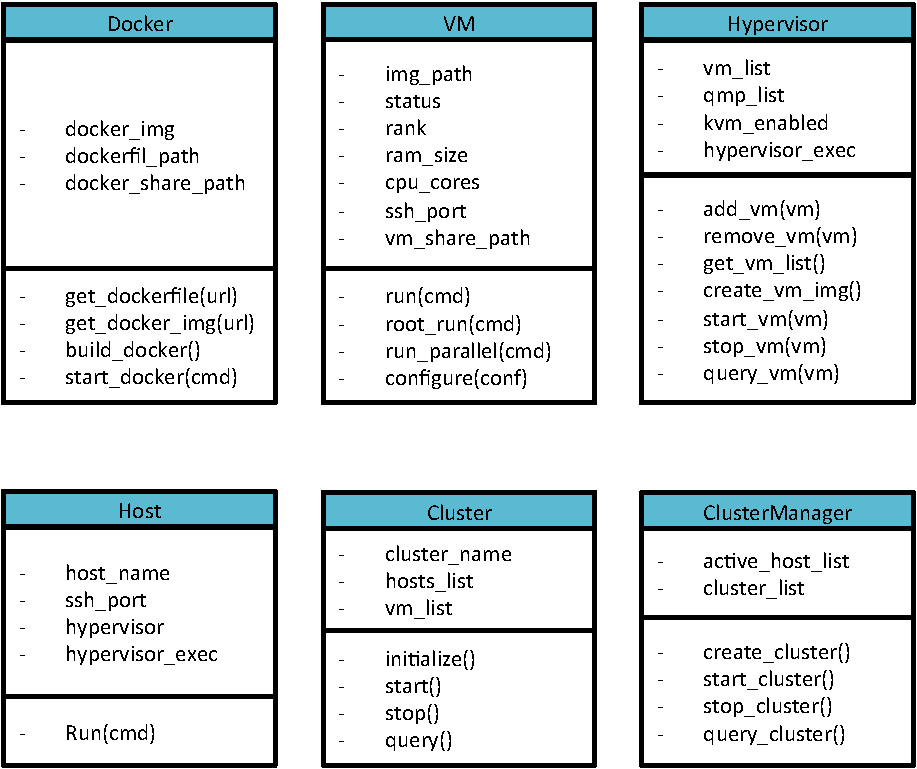
\includegraphics[width=0.5\textwidth]{figures/ood.pdf}
\end{figure}
In this section, we discuss the design details of our BEE framework. To better manage large scale BEE clusters and for extensibility consideration, we choose to use object-oriented design in python for BEE as shown in \textbf{Figure \ref{ood}}. We design several key classes for key components in BEE, including: \texttt{Docker}, \texttt{VM}, \texttt{Hypervisor}, \texttt{Host}, \texttt{Cluster}, and \texttt{ClusterManager}. \texttt{Docker} class stores Docker-related information. For example, Docker image name, Dockerfile path, Docker's running state and directory in Docker that is shared between Dockers. It also contains necessary functions to control or run command in the Docker containers. \texttt{Docker} class stores virtual machine-related information, including the Docker class instant, current hardware configurations, network settings, virtual machine image file path, shared storage directory, etc. It also has necessary functions to control the virtual machine. However, we leave start/stop/query function to the \texttt{Hypervisor} class, since implementation of those functions are hypervisor-specific. \texttt{Hypervisor} class stores hypervisor-related information. For example, the path to the hypervisor binary, KVM availability, and a list of virtual machines that it is currently running. Since we allow different machine to use different hypervisors, we inherent \texttt{Hypervisor} class to get hypervisor class for specific hypervisor. For example, we have a \texttt{QEMU} class that is targeting for QEMU hypervisor. Besides all the functions inherent from \texttt{Hypervisor} class, it also has some QEMU-specific function, like QMP virtual machine monitor functions. \texttt{Host} class maintains all the information of each host, including the host name, username, port number and the hypervisor that is currently running on it. It also has functions used to execute command on the host. \texttt{Cluster} class maintains the information of a virtual BEE cluster, including cluster name,  all host nodes and virtual machines involves, network configuration for this cluster, etc. It also has functions to control and query the cluster. \texttt{ClusterManager} class is used to manage multiple clusters on a computing system. It maintains all the active host nodes on the current system, so that they can be shared between cluster. It provide necessary functions to control each clusters. 
%\jchen{A figure showing all classes' structure will be added}
%\qguan{We will discuss the OOP design and provide the usage of different classes - Qiang Guan}

